\documentclass[12pt,report,2019]{uftpibic}

\usepackage[alf]{abntex2cite}
%\renewcommand{\backrefpagesname}{}
%\renewcommand{\backref}{}
\renewcommand*{\backrefalt}[4]{}

\usepackage{tikz}
\usepackage{multirow}
\graphicspath{{}{images/}{figures/}} 
%-------------------------------------------------------------------------------------------------------------------------%
% Endereço Institucional
%-------------------------------------------------------------------------------------------------------------------------%
\address{109 Norte, Av. Ns 15, ALCNO 14, Bl 04, Sala 207}
\cep{77001-090}
\phone{(63) 3232-8037}
\mail{propesq@uft.edu.br}
\city{Palmas}
%-------------------------------------------------------------------------------------------------------------------------%
% Dados do Projeto
%-------------------------------------------------------------------------------------------------------------------------%
\projecttype{voluntario}
\reporttype{P}
\datainicio{01/03/2017}
\dataconclusao{01/03/2019}

\title{RUTI - Rastreamento Urbano de Transporte Integrado: módulo de comunicação e aquisição de dados veicular}
\advisor{Prof.}{Tiago da Silva}{Almeida}{Ms.}
\author{Matheus Aguiar}{Fagundes}
\campus{Campus Universitário de Palmas -- CUP}
\department{Ciência da Computação}
\local{Campus Universitário de Palmas -- CUP, Bloco III, Sala 09}
\area{Ciências Exatas e da Terra}
\financiamento{}
\grupo{GCC -- Grupo de Computação Cientifica}
\keyword{IoT}
\keyword{Transporte Urbano}
\keyword{Rastreamento}
\keyword{Sistemas Embarcados}
\keyword{Transporte Urbano}
\keyword{Rastreamento}
\keyword{Sistemas Embarcados}
\equipeexecutora{\bf Tiago da Silva Almeida}{\bf Coordenador}
\equipeexecutora{Rafael Lima de Carvalho}{Professor Pesquisador}
\equipeexecutora{Warley Gramacho da Silva}{Professor Pesquisador}
\equipeexecutora{Leonardo Rezende Costa}{Aluno}
\equipeexecutora{Matheus Aguiar Fagundes}{Aluno}
%-------------------------------------------------------------------------------------------------------------------------%
% Para evitar a quebra automática dos Capítulos, descomentar abaixo
%-------------------------------------------------------------------------------------------------------------------------%
%\makeatletter
%\patchcmd{\chapter}{\if@openright\cleardoublepage\else\clearpage\fi}{}{}{}
%\makeatother
%-------------------------------------------------------------------------------------------------------------------------%
\begin{document}

\maketitle
\tableofcontents
\setlength{\parindent}{1.5cm}

\chapter{Introdução}

Grandes centros urbanos trazem grandes desafios à gestão na prestação de serviços de qualidade à população. Um desses desafios é o controle de tráfego devido ao tamanho da frota em grandes centros. Atualmente vivemos uma fase de popularização de projetos que envolvam algum tipo de automação eletrônica. Isso é possível devido aos baixos custos e integração de grande variedades de circuitos acoplados (ou dentro do mesmo encapsulamento, os chamados \textit{System-on-Chip} ou somente SoC), trazendo simplicidade na construção de sistemas automáticos. Logo, surgiu uma linha de pesquisa, chamada \textit{Internet of Things} (IoT), em conjunto com a também simplificada área de desenvolvimento Web. 

A aplicabilidade da metodologia IoT é bastante diversa, podendo ser aplicada também ao controle de tráfego urbano nas grandes cidades. Assim, o objeto desse projeto é desenvolver uma solução baseada em IoT para gerenciamento de frota urbana, especificamente em transporte coletivo. Nosso objetivo é desenvolver um sistema de rastreamento e controle individual de cada veículo, com geolocalização, alimentar uma aplicação web com esses dados e também fornecer informações em tempo real aos usuários. 

Os dados capturados dos veículos podem ser utilizados para tomada de decisão em relação a melhores rotas, gastos globais com o transporte, etc.. Um grande desafio, e foco do projeto, é a melhor tecnologia de troca de dados entre veículos e a aplicação Web, devido ao custo de equipamento mais seguros e rápidos e a baixa qualidade da infraestrutura existente. Portanto, nossos esforços empenham-se no sistema de coleta e gestão de dados da frota veicular.

\vspace{1.5cm}
\chapter{Objetivos}

O objetivo desta iniciação científica é desnevolver um módulo veicular para monitoramento do transporte público. Esse módulo é parte do projeto de pesquisa, o qual foi divido essencialmente em três partes partes principais: módulo do veículo, módulo da estação e servidor de aplicação.

Os objetivos de pesquisa em relação ao módulo veícular podem ser detalhados da seguinte forma:

\begin{itemize}
\item Desenvolvimento e integração dos sub-módulos de comunicação: GPS (\textit{Global Positioning System}), GSM (\textit{Global System for Mobile Communications}) e ZigBee;
\item Desenvolvimento do módulo de \textit{datalogger};
\item Desenvolvimento de circuito de leitura dos níveis de combustível do veículo;
\item Integração dos circuitos dentro de um mesmo módulo para acomplamento ao veículo;
\item Análise de eficiência energética do circuito;
\item Coleta de dados em ambiente controlado.
\end{itemize}

É importante destacar que o trabalho proposto não segue metodologias em camadas como muitos trabalhos da literatura \cite{Moore, Chen}. Isso porque existe o problema da falta de protocolos e arquiteturas padronizadas para criação de projetos caracterizados como IoT, como por exemplo descrito no trabalho de \citeonline{Al-Qaseemi}.

Logo, o objetivo é desenvolver uma arquitetura simplificada para troca de informação com menor latência. Ou seja, o móodulo terá somente duas camadas: uma camada abstrata de aplicação e uma camada abstrata de coleta de dados, sem referência com o modelo OSI (\textit{Open System Interconnection}). 

Como processador, ou como gerenciador, do módulo existem várias opções, como Raspberry \cite{raspberry} ou Photon \cite{photon}. Mas por simplicidade, custo e documentação, será utilizado no projeto a plataforma Arduino \cite{arduino}.

\chapter{Metodologia}

Para o desenvolvimento do projeto serão utilizadas plataformas microcontroladas para gerenciamento da comunicação de dados. Atualmente diversas plataformas baseadas em microcontroladores e SoCs são empregadas em projeto de IoT, e em sua maioria são de código fonte aberto. Por possuir um custo baixo e ampla documentação, escolhemos a plataforma Arduino. A Figura \ref{fig:projeto}, ilustra todas os componentes do projeto, destacado em pontilhado, e as interações entre esses componentes.

\begin{figure}[!htpb]
\centering
\caption{Diagrama de fluxo de dados do projeto destacando os sub-módulos envolvidos e os canais de comunicação em cada etapa.}
%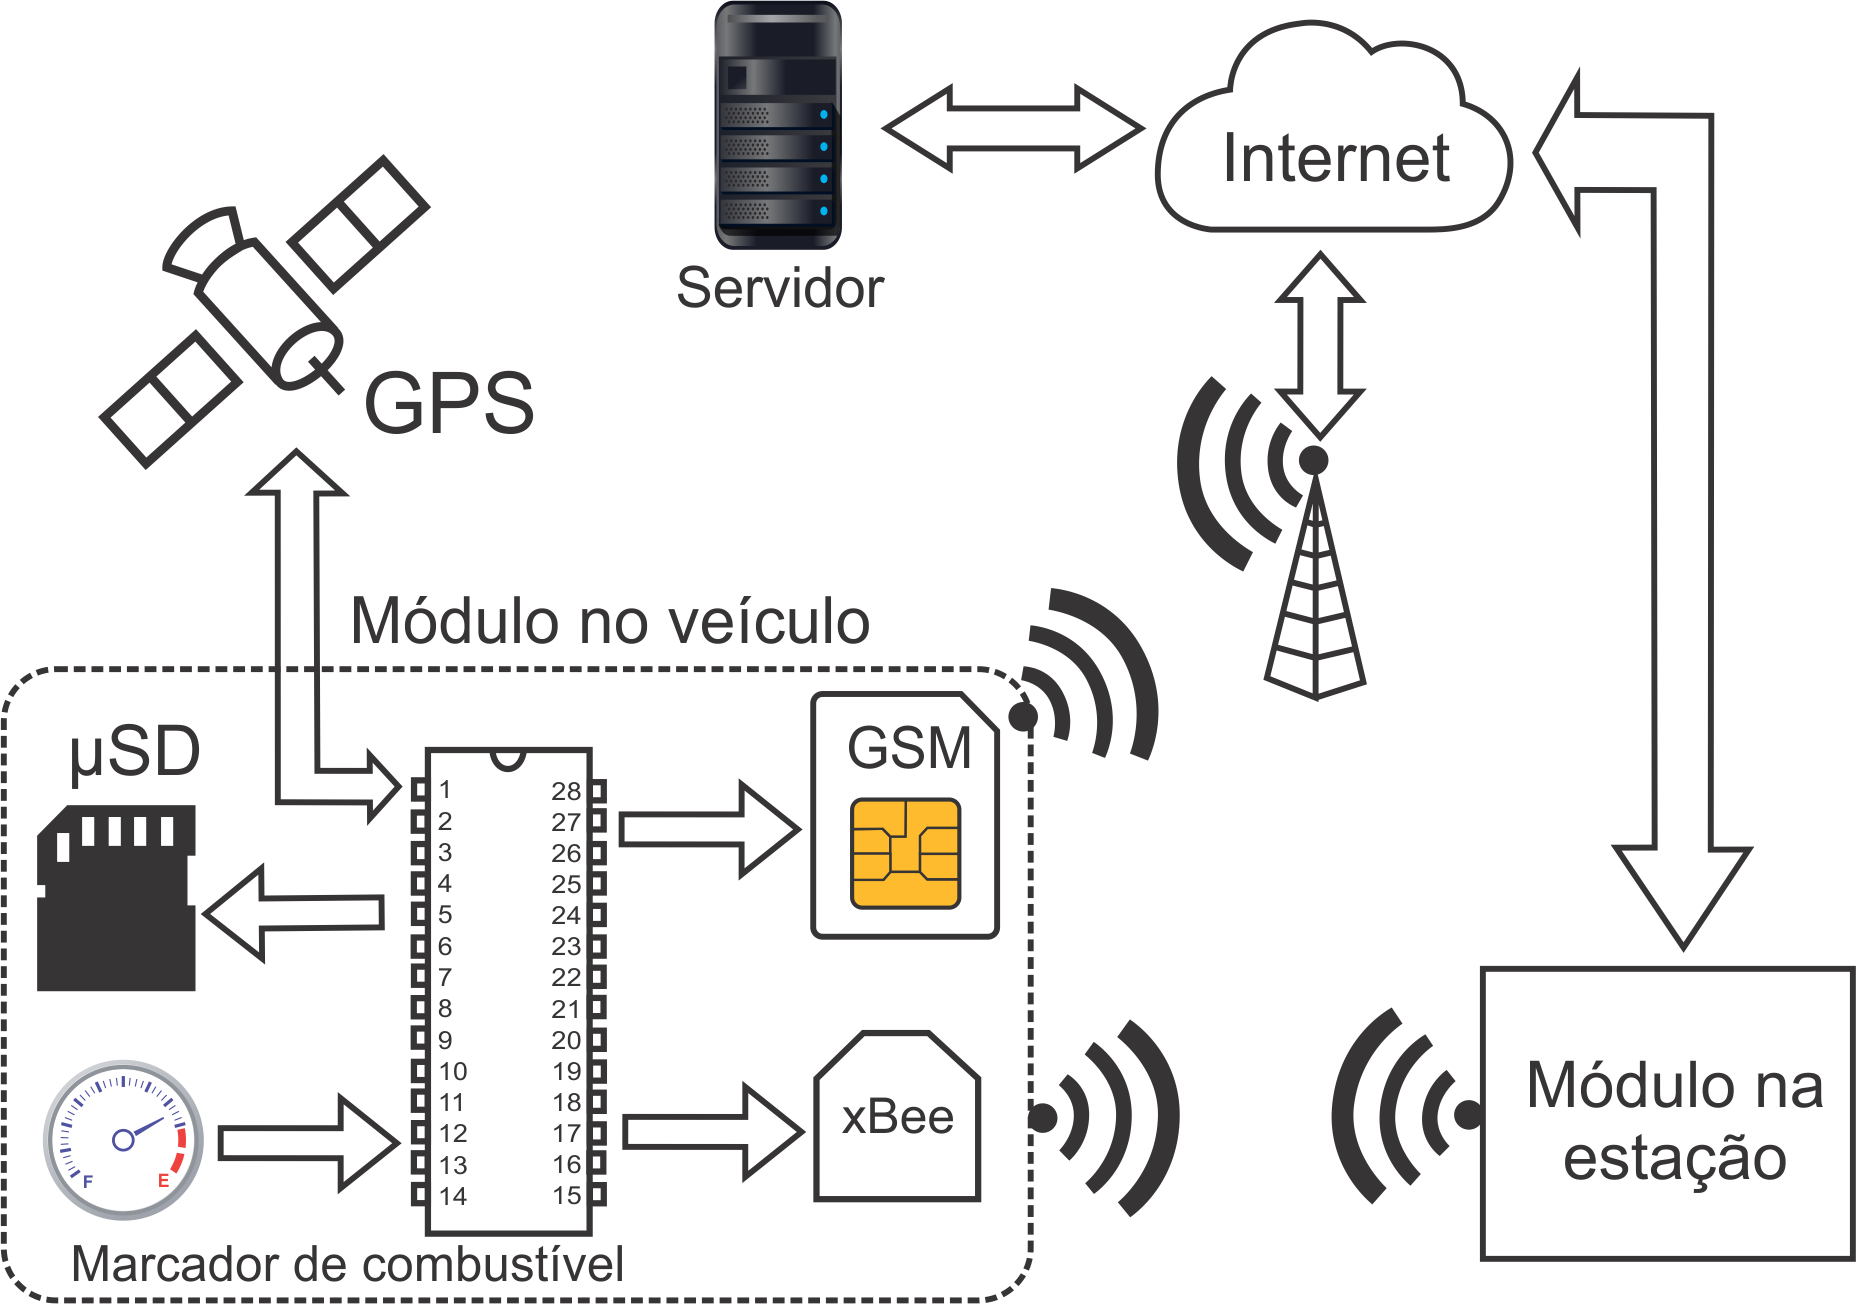
\includegraphics[scale=.8]{ruti1.png}
\label{fig:projeto}
\end{figure}

Objetivo desta iniciação científica é o desenvolvimento do módulo no veículo, ele é o nó central da rede de comunicação sendo gereanciado pelo microcontrolador. Acoplado ao microcontrolador existe três sub-módulos principais para comunicação externa, todos de sendo sem o uso de fios. 

A primeiro é formado pelo sub-módulo GPS que verifica a posição do veículo, em termos de latitude e longitude, e velocidade. O módulo GPS faz a comunicação direta com o satélite, logo, a comunicação nesse ponto é externa ao modelo de rede veicular dentro do nosso projeto. 

O segundo sub-módulo é forma pela comunicação GSM, com foco na rede de dados fornecida pelas operadoras de celulares. O objetivo desse módulo é somente enviar as informações do veículo para um servidor na internet. Essa comunicação é de vital importância para criação de uma base de dados robusta para explorar a análise de tráfego e utilização do transporte público em trabalhos futuros.

O terceiro sub-módulo de comunicação será utilizada a comunicação baseado no padrão IEEE 802.15.4, popularmente conhecido com ``ZigBee''. O padrão IEEE 802.15.4 funciona com altas frequências de operação, comparado à sinais mais comuns como rádio frequência, e baixa taxa de transferência de dados. Objetivo é fornecer protocolos seguros e redundantes para manter a integridade dos dados na comunicação. 

O terceiro sub-módulo será usado na comunicação com a estação ou ponto de ônibus e locais de maior fluxo. Como o sub-módulos GPS e GSM possuem lantências altas de resposta devido a problemas de infraestrutura, o módulo ZigBee fornece os dados ao módulo na estação e estação reenvia e ajusta o sincronismo na linha, de modo a permitir que as dodos no servidor sejam em tempo real.

Além dos sub-módulos de comunicação externa, o módulo do veículo conta com um leitor de cartão de memória, que funcionará como \textit{datalogger}, salvando as informações em caso de falha de comunicação ou outro tipo de falha no veículo e um leitor do nível de combústivel, como por exemplo no trabalho de \citeonline{Lozoya}. 

Como veículos antigos não possuem computador de bordo, o módulo proposto nesse projeto funcionará como sendo um e será de fácil adaptação já que os medidores de combustível são sensores do tipo bóia dentro do tampo ligados a uma resistência elétrica, e por essa variação de resistividade é dado no painel a quantidade de combústivel no tanque. Essa característica permite o acomplamento do módulo proposto sem grandes transtornos. A implementação pode ser feita, se baseando no trabalho de \citeonline{Xu}.

Diferente de trabalho como o de \citeonline{Barcelos}, o projeto proposto não opera com o padrão IEEE 802.11p. O motivo é que essencialmente o padrão IEEE 802.11p opera sobre frequências muita altas para troca de informação entre veículo e estação, e entre veículo e veículo (entre 5,850 GHz e 5,925 GHz nos Estados Unidos e entre 5,860 GHz e 5,900 GHz na Europa). O que dificulta a aquisição de equipamentos de baixo custo. Entretanto, o módulo proposto se carateiza como sendo um equipamento previsto no padrão IEEE 802.11p, o OBU (\textit{On Board Unit}).


Outra ponto importante, é a necessidade de adequar o consumo de energia dos componentes, uma vez que os módulos precisarão ter uma certa autonomia e não necessáriamente funcionará conectado à rede elétrica. Esse é um trabalho que deverá ser feito em fluxo contínuo ao longo do desenvolvimento do protótipo proposto nesse trabalho.

Ao final do projeto, esperamos que haja um protótipo para coleta de dados e já exista dados suficientes para uma disponibilidade e tratamento, os quais poderão ser empregados em algoritmos de heurísticos ou metaheurísticos para análise de tráfego e utilização do transporte coletivo.

\section{O padrão IEEE 802.15.4}

A procura por tecnologias que buscam interligar pontos de acesso de comunicação se tornaram imprescindíveis nos dias atuais. Assim, é necessário um estudo sobre quais tecnologias estão disponíveis para estas operações de comunicação. De acordo com o IEEE, a comunicação sem fio está subdividida nos seguintes protocolos de comunicação: IEEE 802.11 - LAN sem fio ({\it Wireless LAN}), IEEE 802.15 - Wireless Personal Area Network ({\it Bluetooth}), IEEE 802.16 - {\it Broadband Wireless Access} (WiMAX) e IEEE 802.20 - {\it Mobile Broadband Wireless Access} (MobileFi) \cite{marcos}.

Inicialmente a rede deve primeiro ser configurada pelo dispositivo coordenador PAN ({\it Personal Area Network}) e os dispositivos devem associar-se com o PAN. Existem vários parâmetros importantes que são inicializados e armazenados no coordenador do PAN. Alguns são definidos em: comprimento do endereço (curto ou longo), capacidade de segurança e tipo de rede. Uma vez concluído o processo de inicialização, o coordenador PAN entra em modo de espera para receber pedidos de associação \cite{marcos}.

Em uma rede sem semáforos\footnote{O termo semáforo refere-se à um algortimo de controle para entrada de novos dispositivos a rede de modo a evitar que conflitos de entrada entre dispositivos distintos aconteçam.}, um dispositivo que pretenda se associar, primeiro realiza uma busca de detecção de energia no canal. Se o canal estiver ocioso, o dispositivo emite um sinal de solicitação que, simplesmente, verificar se existe um PAN em ação. O coordenador, em seguida, responde com um aviso que incluem muitos parâmetros. Se os parâmetros são compatíveis, o dispositivo envia uma solicitação de associação, que reconhece o coordenador. O dispositivo, em seguida, envia uma solicitação de dados, que é também checada pelo Coordenador. Se o Coordenador aprova, transmite uma associação de resposta, que é reconhecida pelo aparelho. Uma vez que a associação é confirmada pela resposta do MAC, o dispositivo e o coordenador podem iniciar transferências de dados \cite{marcos}.

Um dado PAN pode ser configurado como um sinal de rede ativado ou como não-ativado. Em um sinal de rede ativado, {\it frames} são utilizados para sincronizar dispositivos, identificar o coordenador PAN e estabelecer a necessária superestrutura dentro de uma rede. Esta estrutura ilustra a comunicação do arranjo global de muitos nós da rede, com o tempo de conclusão de cada mensagem (e os avisos opcionais associados). Uma vez que o superframe está dividido em sinais, o superframe inicia com um {\it beacon} (sinal) e é seguido de 16 intervalos (0-15) de tempos iguais, determinando assim o tempo do super {\it frame} \cite{marcos}.

Existem três tipos de transferência de dados suportados:

\begin{itemize}
\item A partir de um coordenador para um dispositivo PAN;
\item A partir de um dispositivo para um coordenador PAN;
\item A partir de um dispositivo para outro dispositivo ponto a ponto.
\end{itemize}

Em uma rede com topologia estrela, apenas os dois primeiros tipos de transferência são utilizados. Estas transações ocorrem de maneira diferente para redes com sinal ativo ({\it Beacon-Enabled}) e para redes com sinal desativado ({\it Non-Beacon-Enabled}), apesar de sinais de quadros sempre serem necessários para a associação.

Um sinal de rede ativo é mais útil para situações em que duração da vida útil da bateria e dados periódicos são necessários. Quando o coordenador for conFigurado como uma rede de sinal ativado, o coordenador FFD ({\it Full Function Device}) envia sinais de transmissão em intervalos regulares. Os dispositivos de funções reduzidas RFDs ({\it Reduce Function Device}) (alimentação por bateria) podem, então, introduzir um baixa potência (sleep) depois de um sinal, e acordar um pouco antes do próximo sinal ocorrer, assim, conservar o tempo de vida da bateria \cite{marcos}. A Figura \ref{fig:xbee} mostra o driagrama esquemático do módulo de conexão do ZigBee com o Arduino (módulo shield).

\begin{figure}[!h]
\centering
%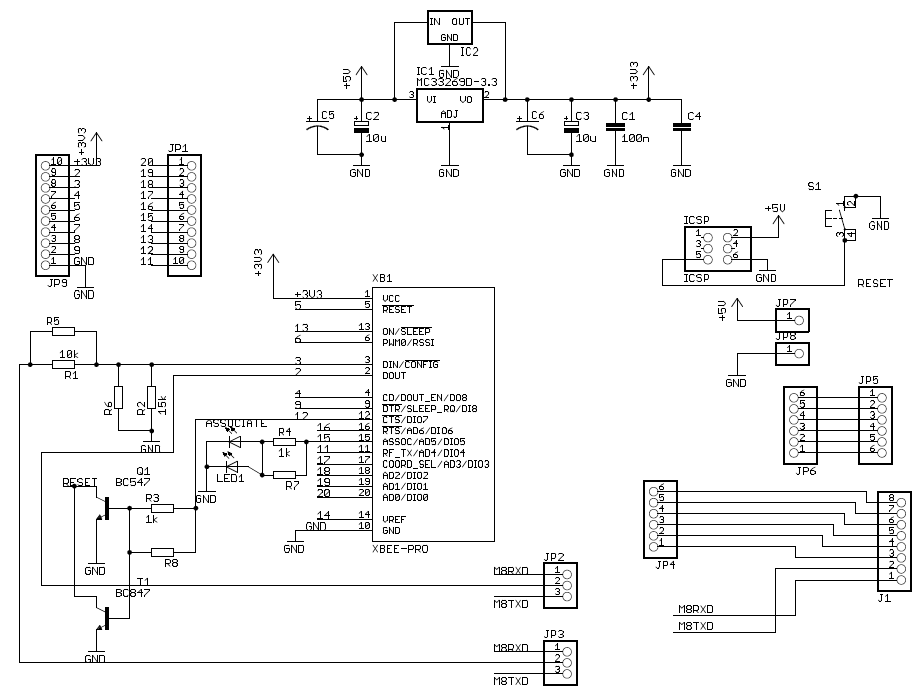
\includegraphics[width=15cm]{xbee_shield.png}
\caption{Diagram esquemático do módulo shield xBee.}
\label{fig:xbee}
\end{figure}

\section{Arduino UNO}

Todo material do Arduino é disponibilizado pelo fabricante, como a IDE ({\it Integrated Development Environment}) de desenvolvimento, bibliotecas e até mesmo o projeto eletrônico das placas são {\it open source}, ou seja, é permitida a utilização e reprodução sem restrição sobre os direitos autorais dos idealizadores do projeto. Porém o nome Arduino, logotipo e o design gráfico de suas placas são registrados e protegidos por direitos autorais \cite{marcos}.

O projeto Arduino é uma plataforma de hardware e software que facilita desenvolvimento de aplicações que utilizam microcontroladores. O Arduino foi criado com o objetivo de facilitar o aprendizado e possibilitar a prototipação e desenvolvimento de projetos com um custo relativamente baixo, além de não exigir um vasto conhecimento em eletrônica. Estes foram sem dúvida os fatores primordiais para a popularização do Arduino em âmbito mundial, não somente entre os desenvolvedores mais experientes, mas também entre os entusiastas e iniciantes \cite{marcos}.

Várias pessoas contribuem com a plataforma, seja na construção de novo hardware ou na confecção de novas bibliotecas e materiais de apoio. O Arduino é uma placa muito eficiente e com recursos necessários para a automação de processos de controle e monitoração. Para o desenvolvimento é utilizado o modelo Arduino Uno R3, que é comumente utilizado em projetos básicos. Existem placas ({\it shields}) voltadas para cada tipo de projeto, permitindo controlar um maior número de dispositivos eletrônicos.

\begin{figure}[!h]
\centering
%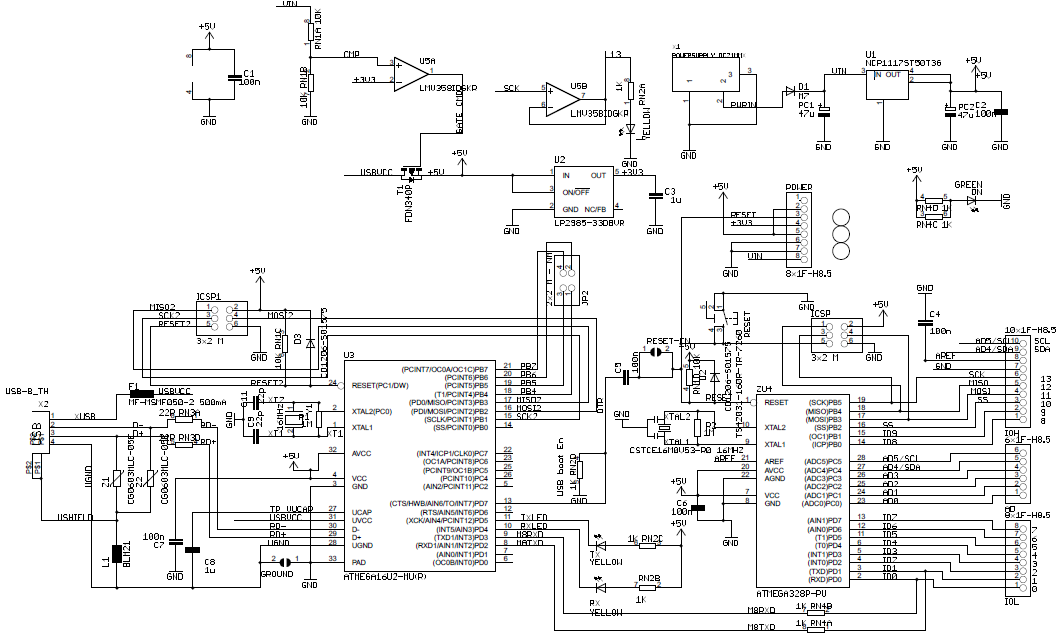
\includegraphics[width=15cm]{arduino.png}
\caption{Diagram esquemático do módulo Arduino.}
\label{fig:arduino}
\end{figure}

O Arduino da Figura \ref{fig:arduino} possui algumas características como:

\begin{itemize}
\item Microprocessador (responsável pelos cálculos e tomada de decisão);
\item Memória RAM (utilizada para guardar dados e instruções, volátil);
\item Memória flash (utilizada para guardar o sotware, não volátil);
\item Temporizadores (timers);
\item Contadores;
\item Clock do sistema.
\end{itemize}

Muitos microcontroladores possuem memória reduzida e menor poder de processamento, característica da maioria dos sistemas embarcados. O Arduino Uno R3, por exemplo, possui as seguintes especificações:

\begin{itemize}
\item Microcontrolador: ATmega328;
\item Portas Digitais: 14;
\item Portas Analógicas: 6;
\item Memória Flash: 32KB (0.5KB usado no bootloader);
\item SRAM: 2KB;
\item EEPROM: 1KB;
\item Velocidade do Clock: 16MHz.
\end{itemize}

O circuito interno do Arduino é alimentado com uma tensão contínua de 5V, isto quando é conectado a uma porta USB do computador. Esta conexão fornece a alimentação e também a comunicação de dados. Caso seja necessário é possível utilizar uma fonte de alimentação externa, que forneça uma saída dentre 7,5 V e 12 V com corrente contínua, ou pode ser ligada diretamente na placa utilizando os pinos Vin e Gnd \cite{marcos}.

\bibliography{bibliografia}

\newpage
\begin{center}
\bf PARECER DO ALUNO A RESPEITO DO PROFESSOR
\end{center}

O professor mostrou-se extremamente responsável para com suas obrigações quanto orientador. Definiu horários semanais para a pesquisa, marcou reuniões (nas quais esteve presente em todas), demonstrou-se prestativo quanto a atendimento fora do horário destinado para o mesmo, estabeleceu meios de comunicação rápidos e eficientes. Proporcionou reuniões com outros orientadores e orientandos para troca de experiência relativa a iniciação cientifica. Mesmo com problemas de saúde fez-se ativo no projeto, não deixando de cumprir suas responsabilidades.  

\begin{center}
\bf PARECER DO PROFESSOR A RESPEITO DO ALUNO
\end{center}

O discente sempre demonstrou grande habilidade com projetos eletrônicos, assim como muita motivação para execução dos trabalhos. A facilidade de assimilação do conteúdo também são características presentes na personalidade do aluno. Único ponto negativo a ressaltar é dificuldade do discente em gerenciar o tempo das atividades. De um modo geral, os alunos apresentam um comportamento de ``hiper participação'' devido ao grande volume de atividades apresentadas. Infelizmente a grande maioria deles não possui maturidade para gerir o próprio tempo e que acarreta em grande atrasos no desenvolvimento das atividades.



\end{document}

